% Version 3.1 December 2024
% JCVHT c05a1271 -- REVISED MANUSCRIPT (28 October 2026)
% Single .tex file (journal forbids \input).
% Campaign of THIS article: 31 PE / 10 s / 3,100 launches.
% Do not mix with the later 100-PE / 9,000-run Access campaign.
% Pin 3.28.98749; DLL SHA-256 prefix 4BBC6270; snapshot tomware_go.
\documentclass[pdflatex,sn-mathphys-num]{sn-jnl}

\usepackage{graphicx}
\usepackage{multirow}
\usepackage{amsmath,amssymb,amsfonts}
\usepackage{amsthm}
\usepackage{mathrsfs}
\usepackage[title]{appendix}
\usepackage{xcolor}
\usepackage{textcomp}
\usepackage{manyfoot}
\usepackage{booktabs}
\usepackage{algorithm}
\usepackage{algorithmicx}
\usepackage{algpseudocode}
\usepackage{listings}
\usepackage{array}
\usepackage{tabularx}
\usepackage{url}

\theoremstyle{thmstyleone}
\newtheorem{theorem}{Theorem}
\newtheorem{proposition}[theorem]{Proposition}
\theoremstyle{thmstyletwo}
\newtheorem{example}{Example}
\newtheorem{remark}{Remark}
\theoremstyle{thmstylethree}
\newtheorem{definition}{Definition}
\raggedbottom

\begin{document}

\title[TOMWare.M Countermeasures]{TOMWare.M: Selective Pintool-Based Countermeasures against Anti-Instrumentation Techniques in Windows Executables}

\author*[1]{\fnm{Francisco S. S.} \sur{Neto}}
\email{francisconeto@icomp.ufam.edu.br}
\author[1]{\fnm{Margefson M.} \sur{Barros}}
\email{margefson.barros@icomp.ufam.edu.br}
\author[1]{\fnm{Eduardo L.} \sur{Feitosa}}
\email{efeitosa@icomp.ufam.edu.br}
\affil*[1]{\orgdiv{Institute of Computing (IComp)}, \orgname{Federal University of Amazonas (UFAM)}, \orgaddress{\city{Manaus}, \state{Amazonas}, \country{Brazil}}}

% ---------------------------------------------------------------------------
% ABSTRACT -- Reviewer Minor 3 + Major 1 (matched timing, not 4080/2081)
% ---------------------------------------------------------------------------
\abstract{Dynamic Binary Instrumentation (DBI) provides fine-grained runtime visibility but exposes artifacts that evasive software may use to identify the analysis environment. This article presents TOMWare.M, an open-source Intel Pin-based \textit{Pintool} implementing five selectively activated countermeasures for debugging indicators, process and module enumeration, Pin-related environment variables, memory-signature comparisons, and timing deviations. Each module was validated with its own controlled detector. A matched timing experiment on \texttt{TestOverhead.exe} ($N=30$, all attempts retained; Table~\ref{tab:timing_matched_n30}) compared Pin with TOMWare loaded and all countermeasures off (TMW0, \texttt{-q}), the same configuration plus artificial overhead (\texttt{-go -q}), and that same overhead with \texttt{SkewMask} (\texttt{-go -do -q}). Conventional medians were $2433.285$, $3083.210$, and $2104.770$ ticks; the fraction of runs at or below the oracle threshold of $3000$ was $30/30$, $11/30$, and $30/30$, respectively. Combined activation (\texttt{-da}) was smoke-tested on the five detectors. Operational compatibility and resource measurements on $31$ Windows PE binaries remain those of the submitted $10\,\mathrm{s}$ protocol; the working-set and CPU percentages in that table are not a performance gain. A controlled demonstrator records a Toolhelp check, an evasive versus work branch, and a hashed output under native / TMW0 / \texttt{-dp}. Five Table~9 x64 benign binaries preserved the same exit code and console milestone under native versus TMW0. Practical recovery of malware or independently protected behavior is not demonstrated. These findings show selective, module-level mitigation of the supported Intel Pin artifacts, with the limitations stated in the evaluation.}

\keywords{Dynamic binary instrumentation, Anti-instrumentation, Intel Pin, Malware analysis, Software protection, Windows executables}

\maketitle

% ===========================================================================
\section{Introduction}
\label{sec:introduction}
% ===========================================================================

Evasive malware and protected executables may alter their behavior according to the environment in which they execute. Operations such as payload decryption, dynamic API resolution, runtime code reconstruction, and the activation of environment-dependent paths may be concealed during static inspection and become observable only at runtime. Dynamic Binary Instrumentation (DBI) is well suited to this context because it enables analysis routines to be inserted into compiled programs without requiring source code, recompilation, or permanent modification of the executable. Intel Pin, for example, provides fine-grained access to instructions, registers, control transfers, function calls, and memory operations \cite{luk2005pin}.

The visibility provided by DBI is accompanied by an observable instrumentation footprint. Dynamic translation and auxiliary analysis routines may introduce memory regions, libraries, processes, internal data structures, environment variables, and additional interactions with the operating system. Instrumentation can also alter execution timing and resource consumption. Evasive programs may inspect these differences through anti-instrumentation checks to determine whether they are executing under analysis. When an instrumentation indicator is detected, a program may terminate, delay execution, follow an alternative path, or suppress relevant behavior. These responses reduce the completeness and fidelity of the evidence collected through dynamic analysis \cite{Rodriguez2016,GiorgioC2022}.

The practical relevance of this problem has been demonstrated at different experimental scales. Polino et al.\ identified at least one anti-instrumentation technique in 15.6\% of 7,006 analyzed samples \cite{polino2017measuring}. Kim et al.\ subsequently examined 763,985 Windows malware samples collected between 2017 and 2020 and reported that an average of 16.21\% employed anti-analysis techniques \cite{kim2022large}. Although the study by Kim et al.\ covers mechanisms beyond DBI detection, its findings reinforce that awareness of the execution environment remains a recurring challenge for automated malware analysis.

Prior research has documented several observation surfaces through which DBI environments can be identified. Santos Filho et al.\ systematized 26 evasion techniques and found that only a subset had corresponding countermeasures documented in the literature \cite{GiorgioC2022}. Park and Park described 24 Windows-oriented detection techniques involving timing overhead, \textit{code-cache} artifacts, memory signatures, Just-in-Time (JIT) compiler characteristics, and environmental indicators \cite{park2024detection}. Lee et al.\ investigated anti-VM and anti-DBI mechanisms employed by commercial software protectors and showed that DBI-based analysis and unpacking require countermeasures against the checks performed by protected code \cite{lee2021bypassing}.

Despite these advances, isolating the effects of individual countermeasures remains an important methodological challenge. Existing approaches commonly emphasize detection coverage or the bypass of checks associated with particular software protectors \cite{polino2017measuring,lee2021bypassing,park2019antidebug}. When multiple protections are enabled simultaneously, an observed functional or operational change cannot be readily attributed to a specific mitigation mechanism. A countermeasure-oriented design, in which each protection can be selectively activated and evaluated, establishes a more direct relationship among the detection surface, the implemented response, and the effects resulting from its activation.

This article presents \textbf{TOMWare.M}\footnote{Source code, controlled detectors, experimental scripts, sample SHA-256 identifiers, and results are available at: \url{https://github.com/TOMWare-analises/TOMWare}. The campaign binary of this article is identified by Intel Pin $3.28.98749$ and \texttt{TOMWare.dll} SHA-256 prefix \texttt{4BBC6270} on guest snapshot \texttt{tomware\_go}. The candidate source tag is \texttt{jcvht-dll-4bbc6270-candidate} (commit \texttt{a22e01d}); that tag is not bit-reproducible.}, an open-source, countermeasure-oriented \textit{Pintool} built on Intel Pin for Windows. TOMWare.M provides five independently selectable countermeasures. \texttt{AntiDebug} normalizes selected PEB-based debugging indicators. \texttt{ProcessEnum} filters configured process and module artifacts through intercepted enumeration and query interfaces. \texttt{SanitizePinEnvVars} sanitizes Pin-related variable names in the process environment block. \texttt{InstMemcmpMask} masks configured DBI signatures when they are exposed through supported memory-comparison routines. Finally, \texttt{SkewMask} compensates for excess delay through selected suspension functions and timing sources.

Because the targeted surfaces expose heterogeneous artifacts, the five countermeasures do not rely on a single intervention mechanism. TOMWare.M combines process-structure normalization, enumeration filtering, environment-block sanitization, comparison-routine wrapping, and timing adjustment. Each module operates within an explicitly defined scope and can be activated independently.

Based on this design, the study addresses the following research questions:

\begin{itemize}
    \item \textbf{RQ1:} To what extent does each TOMWare.M countermeasure suppress its targeted Intel Pin indicator through the monitored interface while preserving the execution of the corresponding controlled detector?
    \item \textbf{RQ2:} What operational compatibility and changes in execution time and resource utilization are observed when each countermeasure is individually applied to benign and malicious Windows executables?
\end{itemize}

The evaluation combines controlled functional validation with a corpus-based operational assessment. Five detector programs served as functional oracles. All five countermeasures achieved their intended outcomes within the monitored interfaces and experimental conditions of those oracles. The quantitative \texttt{SkewMask} claim used in this revision is the matched $N=30$ experiment (Table~\ref{tab:timing_matched_n30}). The originally submitted \texttt{-go} versus \texttt{-do} comparison confounds the artificial-load generator with \texttt{SkewMask} and is retained only in Appendix~\ref{app:timing_confounded}.

Operational compatibility and performance were evaluated using 31 Windows Portable Executable (PE) binaries (17 benign, 14 malware). For each of the 155 binary-countermeasure combinations, the baseline and countermeasure-enabled conditions were each launched ten times in alternating order, totaling 3,100 independent runs under a fixed $10\,\mathrm{s}$ observation window. Compatibility in that campaign means that the profile-specific launch outcome was preserved. It does not mean that each malware sample implemented the corresponding check, nor that enabling a module recovered hidden behavior. The working-set and CPU percentages of the original resource table belong to this $10\,\mathrm{s}$ protocol and are not a performance gain. Combined activation (\texttt{-da}) was smoke-tested on the five detectors; it is not a second $3{,}100$-run campaign.

The main contributions of this work are as follows:

\begin{itemize}
    \item The design and implementation of \textbf{TOMWare.M}, an open-source Intel Pin \textit{Pintool} providing five independently selectable countermeasures against distinct anti-instrumentation surfaces in Windows executables.
    \item A countermeasure-oriented architecture that explicitly associates each detection surface with its mitigation mechanism, supported interfaces, and activation parameter.
    \item A two-level experimental methodology that separates functional validation through controlled detector programs from compatibility and operational measurements across benign and malicious executables.
    \item Empirical evidence from five controlled oracles, a matched timing experiment ($N=30$), wait-model and comparison-family checks, a Module32 fixture, a \texttt{-da} smoke test, $3{,}100$ corpus executions on $31$ PE binaries, a labeled controlled recovery demonstrator, and native-versus-TMW0 progress milestones on five Table~9 x64 benign binaries.
    \item An explicit statement that practical recovery of malware or independently protected behavior is \textbf{not demonstrated}, together with a reproducibility package (source, detectors, scripts, SHA-256 identifiers, CSV/JSON records).
\end{itemize}

The remainder of this article is organized as follows. Section~\ref{sec:background} presents the DBI execution model and related work. Section~\ref{sec:evasive_techniques} describes the targeted surfaces. Section~\ref{sec:architecture} presents the architecture. Section~\ref{sec:countermeasure_implementation} details the five countermeasures, including the revised timing, wait, Module32, comparison-family, and \texttt{-da} evidence. Section~\ref{sec:experimental_evaluation} reports the $31$-PE / $10\,\mathrm{s}$ operational campaign, the controlled recovery demonstrator, and the benign progress milestones. Section~\ref{sec:discussion} discusses findings, the remaining independent-sample gap, and threats to validity. Section~\ref{sec:conclusion} concludes.

% ===========================================================================
\section{DBI Artifacts and Countermeasure Landscape}
\label{sec:background}
% ===========================================================================

\subsection{DBI Execution and Observable Artifacts}

Dynamic Binary Instrumentation enables compiled programs to be observed and modified during execution without source code, recompilation, or permanent modification of the executable \cite{luk2005pin,delia2019sok}. Frameworks such as Intel Pin and DynamoRIO use dynamic translation. In Intel Pin, application code is translated by a JIT engine into a \textit{code cache} \cite{luk2005pin,delia2019sok}. This model provides fine-grained access to instructions, registers, control transfers, function calls, and memory operations, but dynamic translation, code-cache allocation, and auxiliary components introduce observable properties that differ from native execution and are framework- and version-dependent \cite{park2024detection,delia2022evaluating}.

Bruening et al.\ identified code, data, and concurrency as relevant dimensions of transparency and described timing as particularly challenging \cite{bruening2012transparent}. Transparency must be distinguished from compatibility: a program may complete while still identifying the instrumentation environment \cite{delia2019sok,delia2022evaluating}. TOMWare.M therefore distinguishes three evaluation dimensions: functional effectiveness (whether a targeted indicator is suppressed through the monitored surface), operational compatibility (whether activation preserves the expected execution profile), and operational effects (changes in execution time and resource utilization). Successful execution is not treated as evidence of complete transparency.

\subsection{Anti-Instrumentation Surfaces}

D'Elia et al.\ organized DBI observations into timing, code pointers, memory contents and permissions, internal structures, operating-system interactions, exception handling, and translation defects \cite{delia2019sok}. Santos Filho et al.\ distinguished direct from indirect techniques \cite{GiorgioC2022}. Park and Park cataloged 24 Windows-oriented techniques \cite{park2024detection}. TOMWare.M addresses five surfaces: debugging indicators, process and module enumeration, Pin-related environment variables, in-memory signature comparisons, and timing sources. Padhy et al.\ noted that TLS callbacks may execute before the conventional entry point \cite{padhy2025threat}, so countermeasures that target early process state must initialize before those checks.

\subsection{Detection and Countermeasure Approaches}

Falc\'{o}n and Riva introduced eXait \cite{falcon2012dynamic}. Kirsch et al.\ showed that programs can exploit internal Pin characteristics \cite{kirsch2018pwin}. Palmaro and Franchina showed that low-level scanning can reveal DBI components \cite{palmaro2021memory}. D'Elia et al.\ and Park and Park compared artifact exposure across frameworks \cite{delia2022evaluating,park2024detection}.

Countermeasure-oriented systems include Arancino \cite{polino2017measuring}, COBAI \cite{craciun2023cobai}, and Peekaboo \cite{gaber2025peekaboo}. Park et al.\ and Lee et al.\ studied protector-oriented anti-debug and anti-DBI bypasses \cite{park2019antidebug,lee2021bypassing}. Apate and hardware-assisted debugging conceal debugger evidence \cite{shi2017apate,zhang2018transparent}. Kim et al.\ and Norby et al.\ measured prevalence and operational cost of anti-analysis checks \cite{kim2022large,norby2025measurement}. PEMU and LibIHT move observation partly out of process \cite{zeng2015pemu,zhao2025libiht}.

This article does not include an experimental bake-off against Arancino. Public Arancino targets Pin~2.14 and 32-bit binaries; the present campaign uses Pin~$3.28$ and x64. Architectural comparison remains in the related-work discussion; no ranking of coverage, compatibility, or cost is claimed.

The distinguishing focus of TOMWare.M is the explicit association of five surfaces with independently selectable mechanisms, and an evaluation that separates controlled functional validation from operational measurements.

% ===========================================================================
\section{Targeted Anti-Instrumentation Surfaces}
\label{sec:evasive_techniques}
% ===========================================================================

TOMWare.M targets five observation surfaces. Table~\ref{tab:detection_surfaces} summarizes representative inspection mechanisms. The table characterizes the broader surface; exact coverage is in Section~\ref{sec:countermeasure_implementation}.

\begin{table*}[t]
\caption{Targeted anti-instrumentation surfaces and representative inspection mechanisms.}
\label{tab:detection_surfaces}
\centering
\begingroup
\footnotesize
\setlength{\tabcolsep}{3pt}
\renewcommand{\arraystretch}{1.15}
\begin{tabularx}{\textwidth}{@{}
>{\raggedright\arraybackslash}p{0.13\textwidth}
>{\raggedright\arraybackslash}p{0.22\textwidth}
>{\raggedright\arraybackslash}X
>{\raggedright\arraybackslash}p{0.18\textwidth}
@{}}
\toprule
\textbf{Surface} & \textbf{Observable indicator} & \textbf{Representative inspection mechanisms} & \textbf{References} \\
\midrule
Debugger state & PEB fields and debugger-related queries. &
\texttt{IsDebuggerPresent}, \texttt{CheckRemoteDebuggerPresent},
\texttt{NtQueryInformationProcess}, PEB fields. &
\cite{park2024detection,lee2021bypassing,park2019antidebug,norby2025measurement} \\
\addlinespace
Processes and modules & Names, handles, paths of DBI components. &
\texttt{CreateToolhelp32Snapshot}, \texttt{Process32First}/\texttt{Next},
\texttt{Module32First}/\texttt{Next}, \texttt{GetModuleHandle},
\texttt{NtQuerySystemInformation}. &
\cite{polino2017measuring,park2024detection,falcon2012dynamic} \\
\addlinespace
Environment variables & Names or values from the instrumentation loader. &
Environment-query APIs, CRT functions, PEB environment block. &
\cite{GiorgioC2022,polino2017measuring,park2024detection} \\
\addlinespace
Memory signatures & DBI-related names, strings, or regions. &
Direct scanning, \texttt{VirtualQuery}, \texttt{memcmp}, \texttt{wmemcmp},
equivalent routines. &
\cite{delia2019sok,delia2022evaluating,palmaro2021memory} \\
\addlinespace
Timing behavior & Elapsed-time deviations from translation. &
\texttt{QueryPerformanceCounter}, \texttt{GetTickCount}, suspension
functions, \texttt{RDTSC}/\texttt{RDTSCP}. &
\cite{park2024detection,bruening2012transparent,oyama2019rdtsc} \\
\botrule
\end{tabularx}
\endgroup
\end{table*}

\texttt{AntiDebug} covers selected PEB-based indicators and the \texttt{IsDebuggerPresent} response derived from \texttt{BeingDebugged}. Independent \texttt{NtQueryInformationProcess} classes, exception-based checks, and debug registers remain outside direct coverage. \texttt{ProcessEnum} filters configured names through Tool Help and \texttt{GetModuleHandle}; \texttt{NtQuerySystemInformation} and PSAPI remain outside coverage. \texttt{SanitizePinEnvVars} renames startup entries whose names begin with \texttt{PIN}. \texttt{InstMemcmpMask} changes the result of supported comparison routines when the second operand matches a configured signature; it does not overwrite memory. \texttt{SkewMask} accumulates excess delay from intercepted relative suspensions and subtracts it from selected timing sources; direct \texttt{RDTSC}/\texttt{RDTSCP} remain outside coverage.

% ===========================================================================
\section{TOMWare.M Design and Execution Model}
\label{sec:architecture}
% ===========================================================================

TOMWare.M is an open-source, countermeasure-oriented \textit{Pintool} on Intel Pin for Windows~\cite{luk2005pin}. Countermeasure selection uses command-line parameters and does not require recompilation. Figure~\ref{fig:tomware_architecture} presents the workflow.

The controller parses parameters, initializes instrumentation, registers callbacks and replacements, and starts the target under Pin. Parameters \texttt{-dd}, \texttt{-dp}, \texttt{-de}, \texttt{-dm}, and \texttt{-do} activate \texttt{AntiDebug}, \texttt{ProcessEnum}, \texttt{SanitizePinEnvVars}, \texttt{InstMemcmpMask}, and \texttt{SkewMask}. The \texttt{-q} flag loads TOMWare with all five knobs off (TMW0): this is Pin with \texttt{TOMWare.dll} loaded, not bare Pin. EMPTY, when used, is Pin with \texttt{EmptyPinTool.dll}, not Pin without a tool. The \texttt{-da} parameter activates all five countermeasures. Combined activation was smoke-tested on the five controlled detectors (Table~\ref{tab:da_smoke}). That smoke test is not a $3{,}100$-run corpus campaign and does not enable \texttt{-go}.

\begin{figure*}[t]
\centering
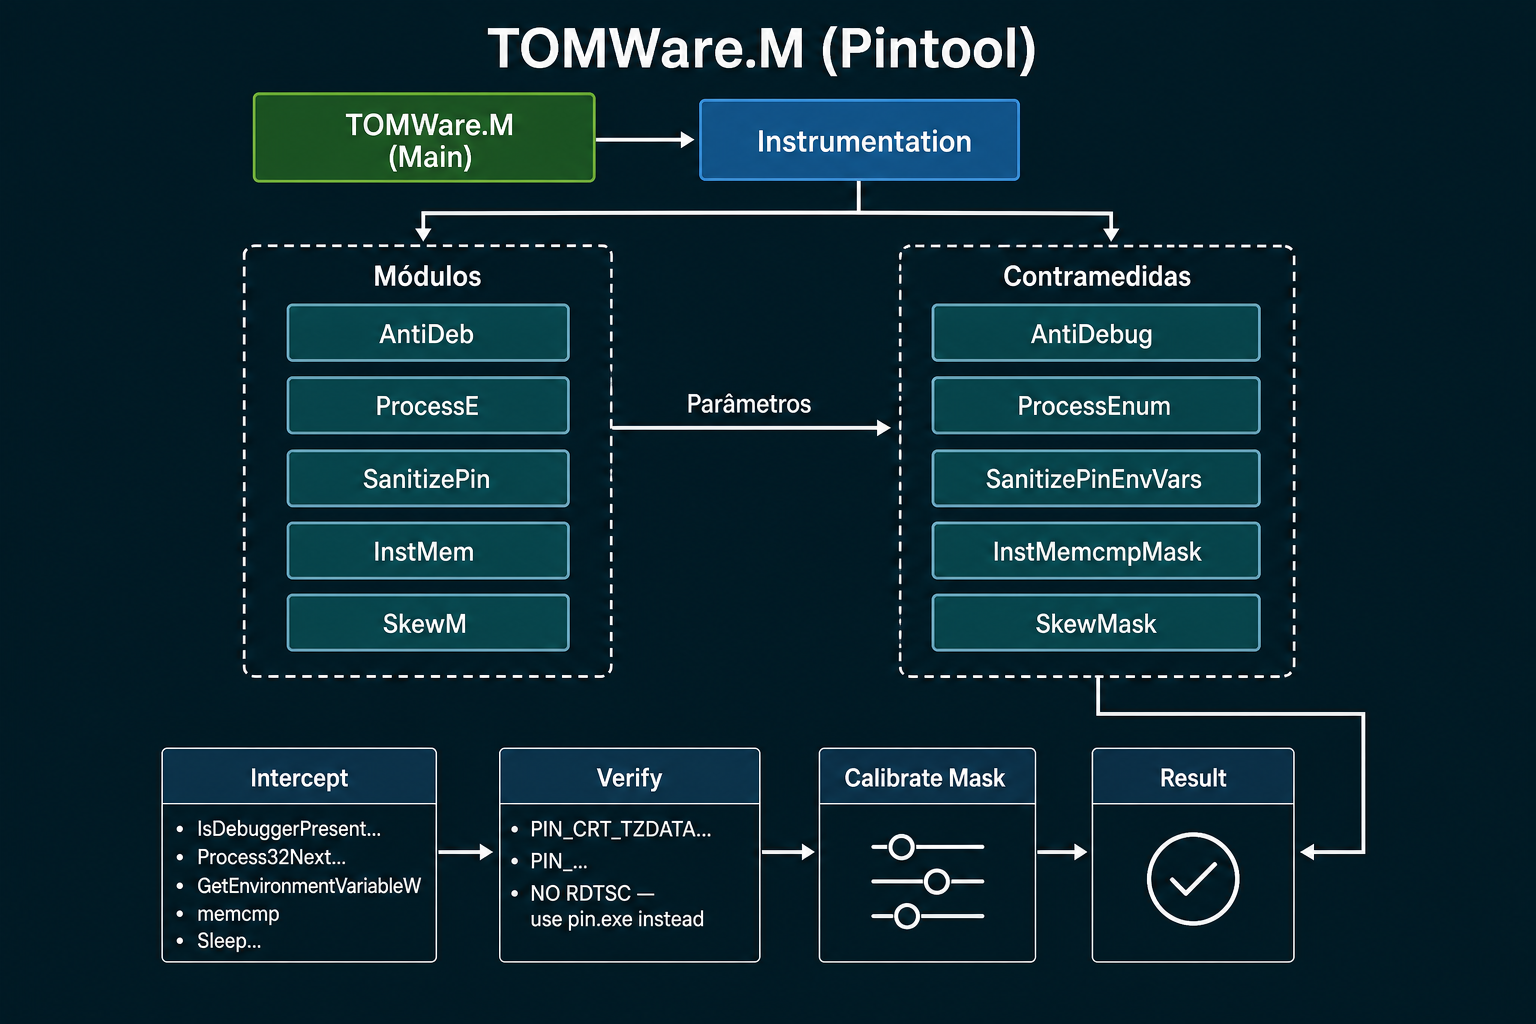
\includegraphics[width=0.96\textwidth,keepaspectratio]{tomwareM.png}
\caption{Countermeasure-oriented architecture and activation workflow of TOMWare.M.}
\label{fig:tomware_architecture}
\end{figure*}

\texttt{AntiDebug} and \texttt{SanitizePinEnvVars} operate on process structures during early initialization. Modules that intercept APIs register image-load callbacks. Experimental orchestration is outside the Pintool core: external scripts launch conditions, collect measurements, and write CSV/JSON records.

% ===========================================================================
\section{Countermeasure Mechanisms}
\label{sec:countermeasure_implementation}
% ===========================================================================

Each subsection states the activation point, monitored interfaces, transformation, functional validation, and boundaries. Successful mitigation through one interface does not imply that equivalent inspections through alternative mechanisms are neutralized.

\subsection{AntiDebug: PEB-Based Debugger-State Normalization}
\label{subsec:antidebug_implementation}

\texttt{AntiDebug} obtains the PEB through the TEB, clears \texttt{BeingDebugged}, and locates \texttt{NtGlobalFlag} at the architecture-specific offset after verifying that the destination is writable. The procedure runs at startup and again when the main image loads. Because \texttt{IsDebuggerPresent} reads \texttt{PEB.BeingDebugged}, clearing that field changes the API result without replacing the function. The implementation does not replace \texttt{CheckRemoteDebuggerPresent} or \texttt{NtQueryInformationProcess}.

Functional validation used \texttt{TestAntiDebug.exe} under the same simulated-debugging stimulus: baseline \texttt{-gdb -q} versus treatment \texttt{-gdb -dd -q}. Table~\ref{tab:antidebug_validation} reports the pair.

\begin{table}[t]
\caption{Functional validation of the \texttt{AntiDebug} countermeasure.}
\label{tab:antidebug_validation}
\centering
\small
\begin{tabularx}{\columnwidth}{@{}Xccc@{}}
\toprule
\textbf{Observed indicator} & \shortstack{\textbf{Baseline}\\\texttt{-gdb -q}} & \shortstack{\textbf{AntiDebug}\\\texttt{-gdb -dd -q}} & \textbf{Effect} \\
\midrule
\texttt{IsDebuggerPresent()} & 1 & 0 & Derived \\
\texttt{PEB.BeingDebugged} & 1 & 0 & Direct \\
\texttt{PEB.NtGlobalFlag} & 1 & 0 & Direct \\
Execution outcome & Complete & Complete & Preserved \\
\botrule
\end{tabularx}
\vspace{3pt}
\parbox{\columnwidth}{\footnotesize Direct: PEB field normalized by the module. Derived: API response affected by \texttt{BeingDebugged}.}
\end{table}

\subsection{ProcessEnum: Process and Module Artifact Filtering}
\label{subsec:processenum_implementation}

\texttt{ProcessEnum} replaces \texttt{Process32First}/\texttt{Next} (A/W) and \texttt{Module32First}/\texttt{Next} (A/W). Matching \texttt{pin.exe} process entries and configured module names (\texttt{pinvm.dll}, \texttt{pinipc.dll}, \texttt{TOMWare.dll}) are skipped; unrelated entries keep their order. \texttt{GetModuleHandleA}/\texttt{W} return a null handle for a matching non-null request and otherwise forward.

The original oracle \texttt{TestProcessEnum.exe} exercises Unicode \texttt{Process32} and \texttt{GetModuleHandleA}. Table~\ref{tab:processenum_validation} remains that oracle. The \texttt{Module32} path had no positive control in the submitted manuscript because the monitored module names were absent from the baseline.

\begin{table}[t]
\caption{Original oracle-level functional validation of \texttt{ProcessEnum} (\texttt{TestProcessEnum.exe}).}
\label{tab:processenum_validation}
\centering
\small
\begin{tabularx}{\columnwidth}{@{}Xccp{0.22\columnwidth}@{}}
\toprule
\textbf{Monitored artifact} & \shortstack{\textbf{Baseline}\\without \texttt{-dp}} & \shortstack{\textbf{ProcessEnum}\\with \texttt{-dp}} & \textbf{Observed effect} \\
\midrule
\texttt{pin.exe} & 8 & 0 & Filtered \\
\texttt{pinvm.dll} & 0 & 0 & Not observed \\
\texttt{pinipc.dll} & 0 & 0 & Not observed \\
\texttt{TOMWare.dll} & 0 & 0 & Not observed \\
Oracle verdict & Alert & OK & Target suppressed \\
\bottomrule
\end{tabularx}
\vspace{3pt}
\parbox{\columnwidth}{\footnotesize ``Not observed'' is not a positive filtering control.}
\end{table}

This revision adds two controls requested by the reviewer. Table~\ref{tab:module32_fixture} uses a dummy file: a copy of \texttt{version.dll} loaded as \texttt{\%TEMP\%\textbackslash pinvm.dll}. That name is a fixture, not a real Pin module. Under \texttt{-dp} and \texttt{-da} the fixture count falls to zero, \texttt{kernel32} remains visible, and enumeration terminates. Table~\ref{tab:processenum_pin_counts} records \texttt{pin.exe} hide/show on the revision guest with one Pin instance at a time.

\begin{table}[t]
\caption{Module32 fixture. A copy of \texttt{version.dll} was loaded as \texttt{\%TEMP\%\textbackslash pinvm.dll} (dummy name, not a real Pin module).}
\label{tab:module32_fixture}
\centering
\small
\begin{tabular}{llcccc}
\toprule
\textbf{Arm} & \textbf{Knobs} & \textbf{count} & \texttt{fixture\_pinvm} & \texttt{kernel32} & \textbf{terminated} \\
\midrule
Native & --- & 32 & 1 & 1 & yes \\
TMW0 & \texttt{-q} & 31 & 1 & 1 & yes \\
\texttt{-dp} & \texttt{-dp -q} & 30 & 0 & 1 & yes \\
\texttt{-da} & \texttt{-da -q} & 30 & 0 & 1 & yes \\
\bottomrule
\end{tabular}
\end{table}

\begin{table}[t]
\caption{\texttt{TestProcessEnum} \texttt{pin.exe} counts on the revision guest (one Pin instance at a time). TMW0 is Pin with TOMWare loaded and knobs off.}
\label{tab:processenum_pin_counts}
\centering
\small
\begin{tabular}{lcc}
\toprule
\textbf{Arm} & \textbf{Knobs} & \texttt{pin.exe} \\
\midrule
Native & --- & 0 \\
TMW0 & \texttt{-q} & 3 \\
\texttt{-dp} & \texttt{-dp -q} & 0 \\
\texttt{-da} & \texttt{-da -q} & 0 \\
\bottomrule
\end{tabular}
\end{table}

\texttt{NtQuerySystemInformation}, PSAPI, parent--child relationships, and names outside the configured list remain outside coverage.

\subsection{SanitizePinEnvVars: Environment-Variable Sanitization}
\label{subsec:environment_sanitization}

At application start the module walks the PEB environment block. When the first three characters of a name match \texttt{PIN} (case-insensitive), it replaces those characters with \texttt{ZZZ}, preserving entry length. The original \texttt{PIN\_} name is no longer resolved; the value remains under \texttt{ZZZ\_}. Table~\ref{tab:environment_validation} uses \texttt{PIN\_CRT\_TZDATA} as the positive control.

\begin{table}[t]
\caption{Paired functional validation of \texttt{SanitizePinEnvVars}.}
\label{tab:environment_validation}
\centering
\small
\begin{tabularx}{\columnwidth}{@{}Xccp{0.19\columnwidth}@{}}
\toprule
\textbf{Oracle observation} & \shortstack{\textbf{Baseline}\\without \texttt{-de}} & \shortstack{\textbf{Sanitized}\\with \texttt{-de}} & \textbf{Effect} \\
\midrule
\texttt{PIN\_CRT\_TZDATA} (block) & Present & Absent & Sanitized \\
\texttt{PIN\_CRT\_TZDATA} (\texttt{\_dupenv\_s}) & Present & Absent & Sanitized \\
\texttt{PIN\_APP\_LD\_LIBRARY\_PATH} & Absent & Absent & Not observed \\
Oracle verdict & Alert & OK & Suppressed \\
Execution outcome & Complete & Complete & Preserved \\
\bottomrule
\end{tabularx}
\end{table}

\subsection{InstMemcmpMask: Memory-Signature Comparison Masking}
\label{subsec:memory_comparison_masking}

The submitted oracle \texttt{TestMemoryScan.exe} compares candidate positions against \texttt{PIN\_}, \texttt{pin.exe}, \texttt{pinvm.dll}, and \texttt{pinipc.dll} through \texttt{memcmp}. Table~\ref{tab:memory_masking_validation} is unchanged: 255 baseline matches fell to 0 under \texttt{-dm}. That experiment validates \texttt{memcmp} only.

\begin{table}[t]
\caption{Paired functional validation of \texttt{InstMemcmpMask} through \texttt{memcmp} (\texttt{TestMemoryScan.exe}).}
\label{tab:memory_masking_validation}
\centering
\small
\begin{tabularx}{\columnwidth}{@{}Xrrc@{}}
\toprule
\textbf{Signature} & \textbf{Baseline} & \textbf{With \texttt{-dm}} & \textbf{Reduction} \\
\midrule
\texttt{PIN\_} & 212 & 0 & 100\% \\
\texttt{pin.exe} & 11 & 0 & 100\% \\
\texttt{pinvm.dll} & 14 & 0 & 100\% \\
\texttt{pinipc.dll} & 18 & 0 & 100\% \\
\midrule
\textbf{Total} & \textbf{255} & \textbf{0} & \textbf{100\%} \\
\bottomrule
\end{tabularx}
\end{table}

Table~\ref{tab:memcmp_family} adds the family check requested by the reviewer. Exercised exports on the campaign guest: \texttt{memcmp}, \texttt{\_memicmp}, and \texttt{RtlCompareMemory} report a match under native/TMW0 and a non-match under \texttt{-dm}/\texttt{-da}. \texttt{RtlEqualMemory} and \texttt{wmemcmp} were not exported (\texttt{NOT\_EXERCISED}). A seven-byte comparison of \texttt{AAAAAAAA} versus \texttt{AAAAAAAB} is equal by construction and is not listed as a tool defect. Presence on the supported-routine list does not imply that the symbol is replaced in every process. The campaign DLL prefix \texttt{4BBC6270} hooked \texttt{\_memicmp\_l} with a three-argument wrapper; that path is not claimed as validated on the campaign binary.

\begin{table}[t]
\caption{Additional comparison exports. \texttt{PASS} = probe reported a match; \texttt{MASKED} = non-match under the hook; \texttt{NOT\_EXERCISED} = symbol not exported on this guest.}
\label{tab:memcmp_family}
\centering
\small
\begin{tabular}{llll}
\toprule
\textbf{Interface} & \textbf{Native / TMW0} & \texttt{-dm} / \texttt{-da} & \textbf{Status} \\
\midrule
\texttt{memcmp} & PASS & MASKED & exercised \\
\texttt{\_memicmp} & PASS & MASKED & exercised \\
\texttt{RtlCompareMemory} & PASS & MASKED & exercised \\
\texttt{RtlEqualMemory} & --- & --- & NOT\_EXERCISED \\
\texttt{wmemcmp} & --- & --- & NOT\_EXERCISED \\
\bottomrule
\end{tabular}
\vspace{3pt}
\parbox{\columnwidth}{\footnotesize A seven-byte comparison of \texttt{AAAAAAAA} versus \texttt{AAAAAAAB} is equal by construction and is not a tool defect. We do not claim the twelve-name supported list as exercised.}
\end{table}

\subsection{SkewMask: Timing-Skew Compensation}
\label{subsec:timing_skew_compensation}

\texttt{SkewMask} replaces \texttt{Sleep}, \texttt{SleepEx}, and \texttt{NtDelayExecution}. For each intercepted relative delay it measures excess
\begin{equation}
\delta_s = \max\bigl(0,\, \Delta t_{\mathrm{obs}} - \Delta t_{\mathrm{req}}\bigr)
\label{eq:skew_sleep}
\end{equation}
and accumulates $\delta_s$. The accumulated duration is subtracted from \texttt{QueryPerformanceCounter}, \texttt{RtlQueryPerformanceCounter}, \texttt{GetTickCount}, \texttt{GetTickCount64}, \texttt{GetSystemTimePreciseAsFileTime}, and \texttt{QueryInterruptTimePrecise}, after conversion to the unit of each interface.

The functional oracle \texttt{TestOverhead.exe} reads \texttt{GetSystemTimePreciseAsFileTime} before and after a $50\,\mathrm{ms}$ \texttt{Sleep}, multiplies the interval (ms) by $40$, and compares the score with
\begin{equation}
T = 1.5 \times (50 \times 40) = 3000.
\label{eq:threshold}
\end{equation}
A score above $T$ is an anomaly. The threshold is oracle-specific.

\subsubsection{Matched timing experiment (revision claim)}

The originally submitted comparison used \texttt{-go} as baseline and \texttt{-do} as treatment. Those modes do not hold the artificial workload fixed, so the reduction from $4080.37$ to $2081.47$ cannot be attributed to \texttt{SkewMask} alone. That table is preserved, with its original numbers, in Appendix~\ref{app:timing_confounded} and is not the quantitative claim of this revision.

The claim used here keeps the workload fixed and reports every attempt (Table~\ref{tab:timing_matched_n30}): TMW0 (\texttt{-q}), GO (\texttt{-go -q}), and GO\_DO (\texttt{-go -do -q}), $N=30$, \texttt{TestOverhead.exe}, conventional median, anomaly if the score exceeds $3000$. TMW0 is Pin with TOMWare loaded and knobs off, not bare Pin.

\begin{table}[t]
\caption{Matched timing oracle, \texttt{TestOverhead.exe}, fixed $N=30$, every attempt retained. Conventional median (mean of the two central values). Anomaly if the score exceeds $3000$.}
\label{tab:timing_matched_n30}
\centering
\small
\begin{tabular}{llrrll}
\toprule
\textbf{Arm} & \textbf{Knobs} & $\mathbf{N}$ & \textbf{Median (ticks)} & \textbf{Min--max} & $\boldsymbol{\le 3000}$ \\
\midrule
TMW0 & \texttt{-q} & 30 & 2433.285 & 2168--2750 & $30/30$ \\
GO (baseline) & \texttt{-go -q} & 30 & 3083.210 & 2722--3845 & $11/30$ \\
GO\_DO (treatment) & \texttt{-go -do -q} & 30 & 2104.770 & 2073--2146 & $30/30$ \\
\bottomrule
\end{tabular}
\vspace{3pt}
\parbox{\columnwidth}{\footnotesize Wilson 95\% intervals: GO $[21.9\%,54.5\%]$; TMW0 and GO\_DO $[88.6\%,100\%]$. Pin $3.28.98749$, DLL prefix \texttt{4BBC6270}. File SHA-256 of the retained series: \texttt{76208218\ldots9827}.}
\end{table}

\begin{figure}[t]
\centering
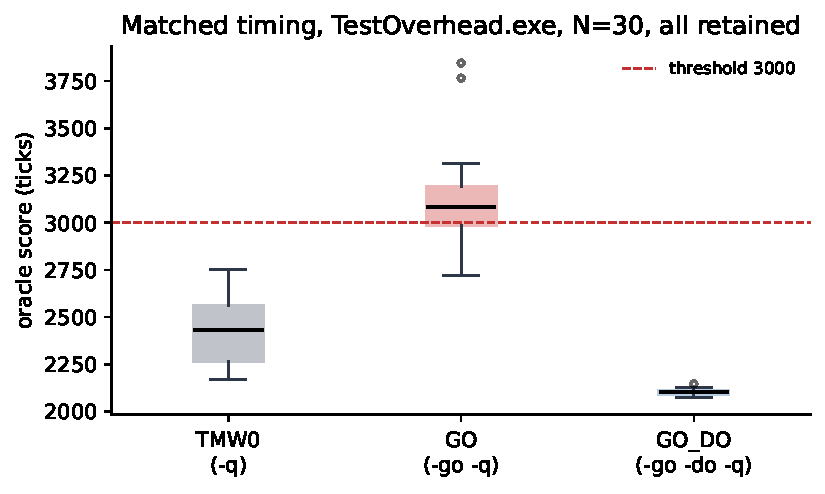
\includegraphics[width=0.92\columnwidth]{timing_n30.pdf}
\caption{Matched timing scores on \texttt{TestOverhead.exe} ($N=30$ per arm, all attempts retained). The dashed line is the oracle threshold of $3000$ ticks. Companion to Table~\ref{tab:timing_matched_n30}.}
\label{fig:timing_n30}
\end{figure}

\subsubsection{Wait model and clock coherence}

A wait-model oracle (\texttt{TestConcurrentWaitsLogged}, $N=5$, no \texttt{-go}; Table~\ref{tab:wait_model_n5}) recorded sequential $2\times 200\,\mathrm{ms}$ sleeps, two concurrent sleeps, a \texttt{TickCount} pair, and an early-returning \texttt{WaitOne}($500\,\mathrm{ms}$). All 20 runs exited 0. The two Sleep intervals still intersected under Pin (median intersection $\sim 207/212/196\,\mathrm{ms}$). The failed predicate is Join-wall $<$ sequential, not serialization of the sleeps. \texttt{WaitOne} does not demonstrate \texttt{SleepEx}. \texttt{SkewMask} does not restore Join-wall $<$ sequential. We do not claim a globally coherent clock under Pin. Timeouts of the same oracle under \texttt{-go} are $10{,}000$ \texttt{\_\_nop} insertions per instruction (\texttt{SimulateOverhead}), not a tool crash.

\begin{table}[t]
\caption{Wait model, \texttt{TestConcurrentWaitsLogged}, $N=5$, no \texttt{-go}. Conventional medians in milliseconds. EMPTY is Pin with an empty pintool. TMW0 is Pin with TOMWare loaded and knobs off.}
\label{tab:wait_model_n5}
\centering
\small
\begin{tabular}{lrrrr}
\toprule
\textbf{Arm} & \textbf{seq $2\times200$} & \textbf{Join wall} & \textbf{Tick+$50$} & \textbf{WaitOne($500$)} \\
\midrule
Native & 406.218 & 213.678 & 62 & 45.867 \\
EMPTY & 433.421 & 571.867 & 62 & 445.610 \\
TMW0 (\texttt{-q}) & 441.209 & 553.862 & 78 & 441.411 \\
\texttt{-do -q} & 414.809 & 517.802 & 56 & 383.428 \\
\bottomrule
\end{tabular}
\end{table}

\begin{figure}[t]
\centering
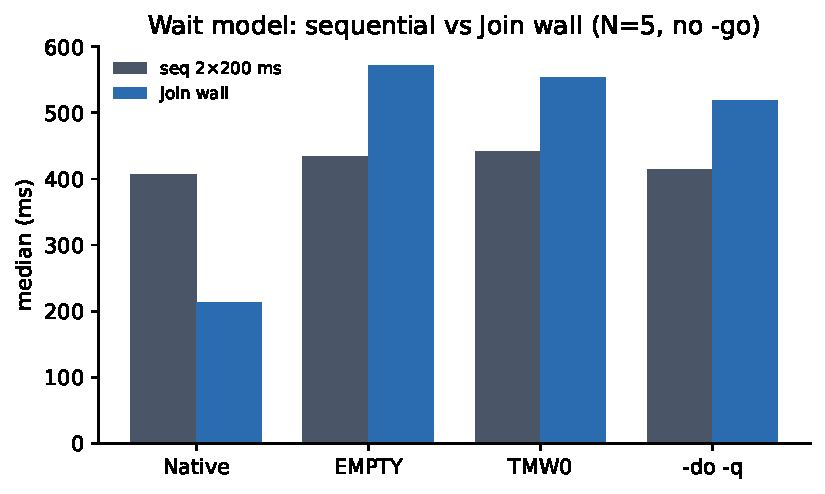
\includegraphics[width=0.92\columnwidth]{wait_join_vs_seq.pdf}
\caption{Join-wall versus sequential $2\times 200\,\mathrm{ms}$ medians (Table~\ref{tab:wait_model_n5}). Under Pin the Join wall exceeds the sequential duration; the two Sleep intervals still overlap. \texttt{SkewMask} does not restore Join-wall $<$ sequential.}
\label{fig:wait_model}
\end{figure}

A later $N=10$ wait series on the same campaign DLL localized two further limitations, which we state rather than treat as resolved. First, \texttt{GetTickCount} can regress on overlapping \texttt{CalibratedSleep} under \texttt{-do} (observed on four of ten overlap runs; QPC did not regress; a burst of clock reads without concurrent sleep did not regress). The cause is the DWORD millisecond truncation of the accumulated skew against a $\sim 15.6\,\mathrm{ms}$ tick quantum. \texttt{SkewMask} was not changed, because a monotonic clamp would invalidate Table~\ref{tab:timing_matched_n30}. Second, \texttt{SleepEx}($500$, alertable) under \texttt{-do} did not return within $180\,\mathrm{s}$ while \texttt{SleepEx}($200$, non-alertable) and a parallel \texttt{Thread.Sleep} did return, and \texttt{OpenThread}+\texttt{QueueUserAPC} succeeded. Remaining active is not proof that every timing-sensitive program works as intended.

Direct \texttt{RDTSC}/\texttt{RDTSCP}, external clocks, and unsupported timing interfaces remain outside coverage.

\subsection{Combined activation (\texttt{-da})}
\label{subsec:da_smoke}

Combined activation was smoke-tested on the five controlled detectors (Table~\ref{tab:da_smoke}). Every detector exited 0. This replaces the submitted sentence that \texttt{-da} was not evaluated. It is not a corpus campaign and does not enable \texttt{-go}.

\begin{table}[t]
\caption{Combined \texttt{-da} smoke test on the five controlled detectors (exit code 0 in every row).}
\label{tab:da_smoke}
\centering
\small
\begin{tabular}{lll}
\toprule
\textbf{Detector} & \textbf{Knobs} & \textbf{Observed} \\
\midrule
\texttt{TestAntiDebug} & \texttt{-gdb -da -q} & PEB/API indicators 0 \\
\texttt{TestProcessEnum} & \texttt{-da -q} & \texttt{pin.exe}=0 \\
\texttt{TestGetEnvironments} & \texttt{-da -q} & \texttt{PIN\_*}=0 \\
\texttt{TestMemoryScan} & \texttt{-da -q} & \texttt{PIN\_}/pin names 0 \\
\texttt{TestOverhead} & \texttt{-da -q} & $2040.7<3000$ \\
\bottomrule
\end{tabular}
\end{table}

% ===========================================================================
\section{Experimental Evaluation and Results}
\label{sec:experimental_evaluation}
% ===========================================================================

This section reports the submitted operational campaign ($31$ PE, $10\,\mathrm{s}$, $3{,}100$ launches) and the revision measurements that answer the reviewer on timing, waits, supported interfaces, and practical benefit. The later $100$-PE / $9{,}000$-run campaign used different windows ($120\,\mathrm{s}$ / $60\,\mathrm{s}$) and is not this protocol; its cells are not imported here.

\subsection{Experimental Environment}
\label{subsec:environment}

Host: 16\,GB RAM, 64-bit Windows 11 Home. VMware Workstation Pro 25H2u1. Guest: 64-bit Windows 10, 8\,GB RAM, four vCPUs, 60\,GB NVMe, host-only network. Snapshot \texttt{tomware\_go} was restored between batches that ran malware. Instrumentation: Intel Pin $3.28.98749$ (x64); \texttt{TOMWare.dll} SHA-256 prefix \texttt{4BBC6270}. Identify that build by the Pin version, the DLL prefix, and the snapshot---not by git hash \texttt{3040df7}.

TMW0 is Pin with that DLL loaded and all five knobs off (\texttt{-q}). The corpus baseline of the submitted campaign is TMW0 versus the single enabled knob. That design measures the incremental effect of activation and does not represent the total overhead of Pin relative to native execution. EMPTY (Pin + empty pintool) appears only in the wait-model table of this revision.

\subsection{Corpus, window, and design}
\label{subsec:corpus}

The corpus comprised 31 Windows PE files: 17 benign applications from a Windows environment and 14 malware samples. Short-lived binaries were those expected to terminate during measurement; persistent binaries were those expected to remain active for the sampling interval. The observation window of this article is $10\,\mathrm{s}$. Table~\ref{tab:corpus} summarizes the design. Complete SHA-256 identifiers are in the reproducibility package. We do not invent VirusTotal family labels.

\begin{table}[t]
\caption{Corpus composition and evaluated binary-countermeasure combinations (this article).}
\label{tab:corpus}
\centering
\small
\begin{tabular}{lrrrr}
\toprule
\textbf{Group} & \textbf{PEs} & \textbf{Short} & \textbf{Persistent} & \textbf{Comb.} \\
\midrule
Benign & 17 & 10 & 7 & 85 \\
Malicious & 14 & 4 & 10 & 70 \\
Total & 31 & 14 & 17 & 155 \\
\bottomrule
\end{tabular}
\end{table}

Each binary was evaluated separately with the five countermeasures. Every combination was executed under baseline and enabled conditions, 10 launches per condition, alternating order: $31\times 5\times 2\times 10 = 3{,}100$ process launches. An additional 260 diagnostic records are preserved but excluded from the consolidated analysis.

Compatibility required natural completion for short-lived binaries and continued process activity during the $10\,\mathrm{s}$ interval for persistent binaries. That criterion is operational. It is not behavioral equivalence, not proof that a sample implemented the corresponding check, and not proof of recovered payload, file, registry, or network activity.

\subsection{Functional validation (consolidated)}
\label{subsec:functional_consolidated}

Table~\ref{tab:oracle_consolidated} consolidates the controlled oracles. The SkewMask row of this table now points to the matched $N=30$ result, not to the confounded $4080$/$2081$ cell.

\begin{table*}[t]
\caption{Consolidated results of the controlled functional oracles. The \texttt{TestProcessEnum} column is wrapped so the name does not collide with the next cell.}
\label{tab:oracle_consolidated}
\centering
\small
\setlength{\tabcolsep}{4pt}
\begin{tabularx}{\textwidth}{@{}
>{\raggedright\arraybackslash}p{0.18\textwidth}
>{\raggedright\arraybackslash}p{0.20\textwidth}
>{\raggedright\arraybackslash}X
>{\raggedright\arraybackslash}X
>{\raggedright\arraybackslash}p{0.18\textwidth}
@{}}
\toprule
\textbf{Module} & \textbf{Oracle} & \textbf{Baseline} & \textbf{Enabled} & \textbf{Validated outcome} \\
\midrule
AntiDebug & \texttt{TestAntiDebug} &
PEB/API indicators equal to one under \texttt{-gdb -q}. &
The three targeted indicators equal to zero under \texttt{-gdb -dd -q}. &
PEB-based indicators normalized. \\
\addlinespace
ProcessEnum & \shortstack[l]{\texttt{TestProcess}\\\texttt{Enum}} &
\texttt{pin.exe} present (original oracle: 8). &
\texttt{pin.exe} absent under \texttt{-dp}. &
Tool Help process entry filtered. \\
\addlinespace
SanitizePinEnvVars & \texttt{TestGetEnvironments} &
\texttt{PIN\_CRT\_TZDATA} resolved. &
Original name not resolved. &
Targeted variable name sanitized. \\
\addlinespace
InstMemcmpMask & \texttt{TestMemoryScan} &
255 matches through \texttt{memcmp}. &
Zero matches through intercepted \texttt{memcmp}. &
Targeted comparisons suppressed. \\
\addlinespace
SkewMask & \texttt{TestOverhead} &
\texttt{-go -q}: $11/30$ scores $\le 3000$ (median $3083.210$). &
\texttt{-go -do -q}: $30/30$ (median $2104.770$). TMW0: $30/30$ (median $2433.285$). &
Matched threshold transition at fixed workload. \\
\bottomrule
\end{tabularx}
\end{table*}

\subsection{Operational compatibility and resource table}
\label{subsec:operational}

Under the adopted operational criterion, every binary-countermeasure combination of the $3{,}100$-run campaign produced the profile-specific launch outcome (completion or continued observation at $10\,\mathrm{s}$). We do not write this as a behavioral-success rate, and we do not treat it as evidence that the 14 malware samples executed the five supported checks.

For each applicable metric the median of the 10 repetitions was calculated per binary. The relative change was
\begin{equation}
\Delta_{\mathrm{rel}}(M) = 100 \times \frac{M_{\mathrm{CM}} - M_{\mathrm{baseline}}}{M_{\mathrm{baseline}}},
\label{eq:rel}
\end{equation}
and the corpus-level value is the median of those per-binary changes. At least one applicable operational metric was available for 144 of the 155 combinations. The remaining 11 involved \texttt{ProcessEnum} (resource collection incomplete) and are not classified as countermeasure failures.

Table~\ref{tab:resources} reprints the submitted resource table so that the numbers remain auditable. The reviewer asked what the large \texttt{SkewMask} cells mean. Remaining alive at a fixed $10\,\mathrm{s}$ window is not equivalent work. A process may wait, follow a different path, or make little progress while still satisfying the compatibility criterion. Those percentages are therefore \textbf{not a performance gain} and are not used as evidence that \texttt{SkewMask} reduced useful work. We cannot attribute the $-87.2\%$ / $-74.4\%$ working-set cells or the $-38.5\%$ / $-29.2\%$ CPU cells to recovered or equivalent progress. A later native-versus-TMW0 recapture of five Table~9 x64 benign binaries (Section~\ref{subsec:prog_benign}) supplies exit-code and console milestones, with parent/child names under TMW0; it does not re-interpret Table~\ref{tab:resources}. Native working-set samples on those five rows were empty because the processes exited in under $3\,\mathrm{s}$; TMW0 peak working set includes Pin. Malware progress remains limited.

\begin{table}[t]
\caption{Median relative changes in operational metrics by corpus group and countermeasure. Protocol of this article: $10\,\mathrm{s}$, $31$ PE. These percentages are not a performance gain.}
\label{tab:resources}
\centering
\small
\begin{tabular}{lrrrrrr}
\toprule
& \multicolumn{2}{c}{Time, short-lived (\%)} & \multicolumn{2}{c}{CPU, persistent (\%)} & \multicolumn{2}{c}{Memory, persistent (\%)} \\
\cmidrule(lr){2-3}\cmidrule(lr){4-5}\cmidrule(lr){6-7}
\textbf{Countermeasure} & Ben. & Mal. & Ben. & Mal. & Ben. & Mal. \\
\midrule
SanitizePinEnvVars & $-3.5$ & $-2.7$ & $+0.2$ & $0.0$ & $0.0$ & $+0.1$ \\
InstMemcmpMask & $-3.9$ & $+0.9$ & $+0.2$ & $+0.3$ & $-1.3$ & $+0.3$ \\
SkewMask & $-0.2$ & N/A & $-38.5$ & $-29.2$ & $-87.2$ & $-74.4$ \\
AntiDebug & $-0.7$ & $+6.8$ & $-0.4$ & $0.0$ & $-0.2$ & $0.0$ \\
ProcessEnum & N/A & N/A & $-7.2$ & $-6.7$ & $-12.8$ & $-7.5$ \\
\bottomrule
\end{tabular}
\vspace{3pt}
\parbox{\columnwidth}{\footnotesize N/A: no group-level median retained. Negative cells describe the $10\,\mathrm{s}$ snapshot, not equivalent progress and not an improvement.}
\end{table}

\subsection{Controlled recovery demonstrator}
\label{subsec:ctrl_pe}

The reviewer asked for a small number of cases with a located check, an observed evasive branch, the matching knob, and additional preserved behavior with a hashed artifact. Import, string, counter, timeout, or ``still alive'' are not that proof. Independent malware and independently protected binaries of this campaign did not supply that chain (Section~\ref{subsec:case_search}). A labeled controlled demonstrator does.

\texttt{TestRecoverWork.exe} (SHA-256 prefix \texttt{5DC7AAC8}) is a benign x64 console program written for this revision. It enumerates processes with \texttt{CreateToolhelp32Snapshot} / \texttt{Process32FirstW} / \texttt{Process32NextW} and compares the image name to \texttt{pin.exe}. If \texttt{pin.exe} is visible it skips the payload and exits 2 (\texttt{EVASIVE}); otherwise it copies a 281-byte input to \texttt{work.bin} and exits 0 (\texttt{WORK}). The expected output hash equals the payload hash (prefix \texttt{DAD7D83B}). Table~\ref{tab:ctrl_pe} records native, TMW0 (\texttt{-q}), and ProcessEnum enabled (\texttt{-dp -q}) on the campaign DLL (prefix \texttt{4BBC6270}), Pin~$3.28.98749$, snapshot \texttt{tomware\_go}, window $30\,\mathrm{s}$. This is a controlled demonstrator, not a malware or protector case; \texttt{identified} remains false in the capture runner.

\begin{table}[t]
\caption{Controlled demonstrator \texttt{TestRecoverWork} (SHA-256 prefix \texttt{5DC7AAC8}). Check: Toolhelp image name \texttt{pin.exe}. Artifact: \texttt{work.bin}, SHA-256 prefix \texttt{DAD7D83B}. Campaign DLL prefix \texttt{4BBC6270}. Not a malware case.}
\label{tab:ctrl_pe}
\centering
\small
\begin{tabular}{lllll}
\toprule
\textbf{Arm} & \texttt{pin.exe} & \textbf{Branch} & \texttt{work.bin} & \textbf{Exit} \\
\midrule
Native & $0$ & WORK & \texttt{DAD7D83B} & $0$ \\
TMW0 (\texttt{-q}) & $1$ & EVASIVE & absent & $2$ \\
\texttt{-dp -q} & $0$ ($144$ calls, $1$ filtered) & WORK & \texttt{DAD7D83B} & $0$ \\
\bottomrule
\end{tabular}
\vspace{3pt}
\parbox{\columnwidth}{\footnotesize Native run \texttt{56c3df9c}; TMW0 \texttt{bd2aa90f}; \texttt{-dp} \texttt{09f1a9d8}. TMW0 wrote no \texttt{work.bin}. The two WORK hashes match the payload. \texttt{pe\_calls\_intercepted}$=144$ is a lead on the intercepted Toolhelp path, not evidence that corpus malware called it.}
\end{table}

\subsection{Benign progress milestones}
\label{subsec:prog_benign}

To clarify the $10\,\mathrm{s}$ resource table, five x64 benign binaries already in the Table~9 catalog were recaptured native versus TMW0 on the same campaign DLL, same snapshot, and the same $10\,\mathrm{s}$ window (Table~\ref{tab:prog_benign}). No extra knob was enabled. Each TMW0 tree contained \texttt{pin.exe}, the sample, and \texttt{conhost.exe}. Exit codes matched on all five rows. BEN\_12 reproduced identical MAKECAB usage text; BEN\_05 reproduced identical MUI stderr; BEN\_10 reproduced the same ``file not found'' message (the drop path differs by run identifier). BEN\_06 and BEN\_16 have empty stdout and are retained only as matching exits. Native peak working set was $0$ because those processes exited before the first sample; TMW0 peak working set includes Pin and is not compared as equivalent application memory. Elapsed time is longer under Pin, as expected. These rows do not re-interpret Table~\ref{tab:resources} as a performance gain. They do not speak to malware progress.

Five leftover i386 binaries from a non-catalog folder produced \texttt{INJECTOR\_ERR\_NO\_ACTIVE\_SERVER} under the campaign \texttt{intel64} Pin and were discarded; they are not Table~\ref{tab:prog_benign}.

\begin{table*}[t]
\caption{Native versus TMW0 progress on five Table~9 x64 benign binaries (window $10\,\mathrm{s}$, DLL prefix \texttt{4BBC6270}). CPU and working set are not treated as comparable work. Not malware recovery.}
\label{tab:prog_benign}
\centering
\small
\begin{tabular}{lllll}
\toprule
\textbf{ID} & \textbf{SHA-256 prefix} & \textbf{Native} & \textbf{TMW0} & \textbf{Milestone} \\
\midrule
BEN\_05 & \texttt{0244aa82} & exit $1$, $2.7\,\mathrm{s}$ & exit $1$, $8.5\,\mathrm{s}$ & identical stderr (MUI $15100$) \\
BEN\_06 & \texttt{0436f442} & exit $3$, $0.5\,\mathrm{s}$ & exit $3$, $7.0\,\mathrm{s}$ & matching exit only \\
BEN\_10 & \texttt{06418110} & exit $0$, $0.5\,\mathrm{s}$ & exit $0$, $2.7\,\mathrm{s}$ & same ``file not found'' stdout \\
BEN\_12 & \texttt{070a98b4} & exit $0$, $0.4\,\mathrm{s}$ & exit $0$, $2.6\,\mathrm{s}$ & identical MAKECAB stdout \\
BEN\_16 & \texttt{07c1f3b3} & exit $0$, $0.4\,\mathrm{s}$ & exit $0$, $3.3\,\mathrm{s}$ & matching exit only \\
\bottomrule
\end{tabular}
\vspace{3pt}
\parbox{\textwidth}{\footnotesize Native runs \texttt{da72342a}, \texttt{7e5629b9}, \texttt{82c51390}, \texttt{5c606d6c}, \texttt{b4ec5812}; TMW0 \texttt{15e9a811}, \texttt{e8f73d32}, \texttt{e880dc03}, \texttt{a01c59b4}, \texttt{0efa955c}. Knobs \texttt{-q -mc 1}. \texttt{json\_ok}$=0$ is expected with ProcessEnum off.}
\end{table*}

\subsection{Independent-sample search (not demonstrated)}
\label{subsec:case_search}

A static IAT/string scan of the 31 PE binaries of this article left \texttt{identified=false} on every row. MAL\_08 and MAL\_13 import \texttt{CreateToolhelp32Snapshot}/\texttt{Process32Next} but contain no standalone \texttt{pin.exe} string. Under the campaign DLL (SHA-256 prefix \texttt{4BBC6270}) a later diagnostic gate with \texttt{-dp -q -mc} classified MAL\_08 as \texttt{INCONCLUSIVE\_ABNORMAL\_EXIT} with a valid counter log and a measured zero (\texttt{pe\_calls\_intercepted}=0), and MAL\_13 as \texttt{INCONCLUSIVE\_NO\_COUNTER\_LOG} (timeout; JSON not flushed). The NAT / TMW0 / TMW\_DP triad was not launched for those two rows.

An in-memory static scan of an extended catalog (2000 benign PE and 1904 AES-zipped infected PE; no host execution) found no standalone \texttt{pin.exe}/\texttt{pinvm}/\texttt{pinipc} string. Apparent \texttt{pin.exe} hits were the substring \texttt{kingpin.exe}. Extra executables with a Toolhelp import or a file-writing profile (Table~\ref{tab:extra_search}) did not yield an intercepted \texttt{Process32}/\texttt{Module32} comparison against a Pin indicator, nor a hashed extra artifact under native versus TMW0. Interactive protected binaries that failed for inverted debugger checks, multi-process hangs under \texttt{-follow\_execv}, or Pin-environment/integrity messages (rather than a located PEB or Toolhelp branch) were discarded and are not listed as cases. Collection failures remain inconclusive: they do not prove absence of evasion and they do not prove countermeasure success.

The only positive hide/show of \texttt{pin.exe} on an existing detector remains the controlled oracle \texttt{TestProcessEnum} (revision guest: $147$ intercepted calls, $1$ filtered; a later repeat on the same DLL recorded $143/1$). That oracle is not a malware case. The \texttt{TestRecoverWork} chain in Table~\ref{tab:ctrl_pe} is a written demonstrator, not an independent sample.

Four earlier candidates (Table~\ref{tab:case_attempt}) were run native / TMW0 / \texttt{-do} for $60\,\mathrm{s}$. Every row had \texttt{new\_files}=0 and empty stdout. They are not case studies.

\begin{table}[t]
\caption{Case-study attempt (knob \texttt{-do}, window $60\,\mathrm{s}$). Every row had \texttt{new\_files}=0 and empty stdout. These binaries are not claimed as successful case studies.}
\label{tab:case_attempt}
\centering
\small
\begin{tabular}{llll}
\toprule
\textbf{Sample} & \textbf{Native} & \textbf{TMW0 (\texttt{-q})} & \texttt{-do -q} \\
\midrule
MAL\_03 & timeout $60\,\mathrm{s}$ & access violation $0\mathrm{xC}0000005$ & timeout \\
MAL\_07 & exit 0 ($\sim 1.4\,\mathrm{s}$) & access violation $0\mathrm{xC}0000005$ & timeout \\
MAL\_10 & timeout $60\,\mathrm{s}$ & timeout & timeout \\
BEN\_06 & exit 3 ($\sim 1.0\,\mathrm{s}$) & exit 3 ($\sim 3.8\,\mathrm{s}$) & timeout \\
\bottomrule
\end{tabular}
\end{table}

\begin{table*}[t]
\caption{Additional practical-benefit search on the campaign DLL (prefix \texttt{4BBC6270}). None of these rows is a case study.}
\label{tab:extra_search}
\centering
\small
\begin{tabular}{llll}
\toprule
\textbf{Candidate} & \textbf{Protocol} & \textbf{Observation} & \textbf{Case?} \\
\midrule
MAL\_08 & Gate \texttt{-dp -q -mc} & Valid JSON; \texttt{pe\_calls}=0; abnormal exit & No \\
MAL\_13 & Gate \texttt{-dp -q -mc} & No counter log (timeout) & No \\
BEN\_41 (\texttt{MpSigStub}) & Gate \texttt{-dp -q -mc} & Valid JSON; \texttt{pe\_calls}=0; HRESULT \texttt{0x80070647} & No \\
SHA \texttt{36685EFC} (corpus) & Native vs TMW0, $60\,\mathrm{s}$ & Both exit 1; $0$ new files; TMW0 \texttt{pe\_calls}=0 & No \\
\texttt{TestProcessEnum} & Smoke \texttt{-dp} & $147$ then $143$ calls, $1$ filtered & Oracle only \\
\bottomrule
\end{tabular}
\vspace{3pt}
\parbox{\textwidth}{\footnotesize SHA \texttt{36685EFC} is one of the 14 malware hashes of this article. Native $\sim 1.5\,\mathrm{s}$, TMW0 $\sim 3.5\,\mathrm{s}$; the extra time is Pin, not a recovered payload. IAT \texttt{IsDebuggerPresent} was not treated as a located branch. Knob \texttt{-dd} was not applied.}
\end{table*}

Practical recovery of suppressed malware or independently protected behavior is \textbf{not demonstrated}. Attempts that failed to collect a check, branch, and hashed extra artifact remain inconclusive.

\subsection{Summary of the research questions}
\label{subsec:rq_summary}

Regarding RQ1, each countermeasure suppressed its targeted indicator on the interface exercised by its oracle. The \texttt{SkewMask} claim is $11/30$ versus $30/30$ at fixed workload (Table~\ref{tab:timing_matched_n30}), not the confounded $4080$/$2081$ cell. Module32, comparison-family, wait-model, and \texttt{-da} evidence is as in Section~\ref{sec:countermeasure_implementation}. Concurrent waits do not yield a globally coherent clock; alertable \texttt{SleepEx} under \texttt{-do} is a stated limitation.

Regarding RQ2, the $10\,\mathrm{s}$ / $31$-PE campaign preserved the operational launch profile of each combination. Resource percentages, including the large \texttt{SkewMask} cells, are not a performance gain. Five Table~9 x64 benign binaries later showed matching native versus TMW0 exits and, on three rows, matching console text (Table~\ref{tab:prog_benign}). Practical benefit on independent malware or protected binaries was not shown.

% ===========================================================================
\section{Discussion}
\label{sec:discussion}
% ===========================================================================

\subsection{Interpretation}

RQ1 is answered within the interfaces, signatures, and conditions of the controlled oracles. The modules reduce indicator visibility without necessarily removing the underlying artifacts: environment entries are renamed, comparison results are forced to non-match, process names are filtered, PEB fields are cleared. Alternative APIs, copied data, direct scans, and unsupported paths may still expose equivalent artifacts.

RQ2 is answered as an operational measurement. Preserving a launch profile is not behavioral equivalence. The large resource cells under \texttt{SkewMask} are consistent with a changed execution state in a short fixed window, not with a demonstrated reduction of useful work.

\subsection{What a malware analyst obtains}

On a binary that actually calls a supported check, the corresponding knob can hide that indicator on the intercepted interface: the oracles show this for PEB fields, \texttt{pin.exe} through Tool Help, \texttt{PIN\_} names, \texttt{memcmp} signatures, and the matched timing oracle. The \texttt{TestRecoverWork} demonstrator (Table~\ref{tab:ctrl_pe}) records that chain on a written Toolhelp check: native and \texttt{-dp} produce the same hashed file; TMW0 takes the evasive branch and writes nothing. On the 14 malware samples of this article we did not locate such a check, did not observe the evasive branch, and did not recover an extra hashed artifact. A later static catalog scan, Toolhelp gates, a native/TMW0 recapture of corpus SHA \texttt{36685EFC}, and discarded protected executables did not change that independent-sample conclusion (Section~\ref{subsec:case_search}). The analyst therefore obtains a selective Pintool whose mechanisms are validated on detectors and one labeled demonstrator, not a demonstrated unpack/drop/C2 gain on this corpus.

\subsection{Limitations and threats to validity}
\label{subsec:limitations}

Implementation coverage is bounded: \texttt{AntiDebug} does not cover independent debugger APIs; \texttt{ProcessEnum} does not intercept \texttt{NtQuerySystemInformation} or PSAPI; \texttt{SanitizePinEnvVars} does not delete values; \texttt{InstMemcmpMask} requires a replaced routine, second-operand match, and expected length; \texttt{SkewMask} does not cover \texttt{RDTSC}/\texttt{RDTSCP}. The wait-model does not give a globally coherent concurrent clock; \texttt{GetTickCount} can regress under overlapping calibrated sleeps; alertable \texttt{SleepEx} under \texttt{-do} may not return.

Construct validity: oracles are deterministic detectors, not commercial protectors. Their outputs must not be read as evidence that corpus binaries executed the same techniques.

Compatibility verifies completion or continued observation, not system-call sequences, coverage, files, registry, or network. Table~\ref{tab:prog_benign} pairs native versus TMW0 exits and console text on five benign binaries; it does not pair comparable CPU or application working set, and it does not cover malware. Medians in Table~\ref{tab:resources} remain descriptive. The baseline is incremental (TMW0 versus one knob), not native-versus-Pin. External validity is limited by 31 x64 PE files, Windows~10, Pin~$3.28.98749$, and a virtualized guest. There is no experimental ranking versus Arancino.

% ===========================================================================
\section{Conclusion and Future Work}
\label{sec:conclusion}
% ===========================================================================

This article presented TOMWare.M, a countermeasure-oriented Pintool on Intel Pin for Windows, with five independently selectable modules.

The controlled oracles showed targeted suppression on the exercised interfaces. The revised timing claim is the matched $N=30$ series ($11/30$ versus $30/30$ at or below $3000$ ticks). Wait-model, Module32 fixture, comparison-family, and \texttt{-da} smoke evidence are included. The $31$-PE / $10\,\mathrm{s}$ / $3{,}100$-launch campaign remains the operational measurement of this article; its resource percentages are not a performance gain. A labeled demonstrator recovers a hashed file when ProcessEnum hides \texttt{pin.exe}; five Table~9 x64 benign binaries keep the same exit and, where present, the same console text under native versus TMW0. Practical recovery of malware or independently protected behavior suppressed by an identified check is not demonstrated.

Future work that remains open: additional debugger and native enumeration interfaces; \texttt{RDTSC}/\texttt{RDTSCP}; a coherent treatment of overlapping and alertable waits if \texttt{SkewMask} is changed (that change would require repeating Table~\ref{tab:timing_matched_n30}); behavioral fidelity by API traces and coverage; a 32-bit TOMWare plus Pin \texttt{ia32} corpus; and---if a real malware or independently protected sample with a located check is obtained---a case study with check, branch, knob, and hashed artifact. Combined activation on the detectors is no longer listed as unevaluated. An Arancino bake-off would require a shared 32-bit protocol and is not claimed here.

TOMWare.M is an experimental platform for bounded countermeasures against Intel Pin detection, treating functional effectiveness, operational compatibility, and instrumentation effects as related but distinct properties.

% ===========================================================================
\begin{appendices}
\section{Originally submitted timing comparison}
\label{app:timing_confounded}

\textit{Note (revision).} This is the originally submitted protocol. The \texttt{-go} versus \texttt{-do} contrast confounds the artificial-load generator with \texttt{SkewMask}. It is retained for traceability and is not the quantitative claim of this revision. The matched comparison is Table~\ref{tab:timing_matched_n30}.

\begin{table}[h]
\caption{Originally submitted functional validation of \texttt{SkewMask} (confounded modes).}
\label{tab:timing_old}
\centering
\small
\begin{tabular}{lcc}
\toprule
\textbf{Metric} & \textbf{Baseline \texttt{-go}} & \textbf{SkewMask \texttt{-do}} \\
\midrule
Oracle score & $4080.37$ & $2081.47$ \\
Calibrated threshold & $3000$ & $3000$ \\
Distance from threshold & $+1080.37$ & $-918.53$ \\
Threshold classification & Above & Below \\
Oracle verdict & Anomaly & No anomaly \\
Execution outcome & Complete & Complete \\
\bottomrule
\end{tabular}
\vspace{3pt}
\parbox{\columnwidth}{\footnotesize A positive distance is above the threshold. The $\approx 49\%$ score difference describes two operational modes and is not a general overhead reduction.}
\end{table}

\end{appendices}

\providecommand{\doi}[1]{\url{https://doi.org/#1}}
\begin{thebibliography}{23}

\bibitem{luk2005pin}
Luk, C.-K., Cohn, R., Muth, R., Patil, H., Klauser, A., Lowney, G., Wallace, S., Reddi, V.J., Hazelwood, K.:
Pin: Building customized program analysis tools with dynamic instrumentation.
In: PLDI '05, pp. 190--200. ACM, New York (2005).
\doi{10.1145/1065010.1065034}

\bibitem{Rodriguez2016}
Rodr\'{\i}guez, R.J., Rodr\'{\i}guez-Gast\'{o}n, I., Alonso, J.:
Towards the detection of isolation-aware malware.
IEEE Latin America Transactions \textbf{14}(2), 1024--1036 (2016).
\doi{10.1109/TLA.2016.7437254}

\bibitem{GiorgioC2022}
Santos Filho, A., Rodr\'{\i}guez, R.J., Feitosa, E.L.:
Evasion and countermeasures techniques to detect dynamic binary instrumentation frameworks.
Digital Threats: Research and Practice \textbf{3}(2), 1--28 (2022). Article 11.
\doi{10.1145/3480463}

\bibitem{polino2017measuring}
Polino, M., Continella, A., Mariani, S., D'Alessio, S., Fontana, L., Gritti, F., Zanero, S.:
Measuring and defeating anti-instrumentation-equipped malware.
In: DIMVA 2017. LNCS, vol. 10327, pp. 73--96. Springer, Cham (2017).
\doi{10.1007/978-3-319-60876-1_4}

\bibitem{kim2022large}
Kim, M., Cho, H., Yi, J.H.:
Large-scale analysis on anti-analysis techniques in real-world malware.
IEEE Access \textbf{10}, 75802--75815 (2022).
\doi{10.1109/ACCESS.2022.3190978}

\bibitem{park2024detection}
Park, S., Park, Y.:
Detection techniques for DBI environment in Windows.
Electronics \textbf{13}(5), 871 (2024).
\doi{10.3390/electronics13050871}

\bibitem{lee2021bypassing}
Lee, Y.B., Suk, J.H., Lee, D.H.:
Bypassing anti-analysis of commercial protector methods using DBI tools.
IEEE Access \textbf{9}, 7655--7673 (2021).
\doi{10.1109/ACCESS.2020.3048848}

\bibitem{park2019antidebug}
Park, J., Jang, Y.-H., Hong, S., Park, Y.:
Automatic detection and bypassing of anti-debugging techniques for Microsoft Windows environments.
Advances in Electrical and Computer Engineering \textbf{19}(2), 23--28 (2019).
\doi{10.4316/AECE.2019.02003}

\bibitem{delia2019sok}
D'Elia, D.C., Coppa, E., Nicchi, S., Palmaro, F., Cavallaro, L.:
SoK: Using dynamic binary instrumentation for security (and how you may get caught red handed).
In: Asia CCS '19, pp. 15--27. ACM, New York (2019).
\doi{10.1145/3321705.3329819}

\bibitem{delia2022evaluating}
D'Elia, D.C., Invidia, L., Palmaro, F., Querzoni, L.:
Evaluating dynamic binary instrumentation systems for conspicuous features and artifacts.
Digital Threats: Research and Practice \textbf{3}(2), 1--13 (2022). Article 10.
\doi{10.1145/3478520}

\bibitem{bruening2012transparent}
Bruening, D., Zhao, Q., Amarasinghe, S.:
Transparent dynamic instrumentation.
In: VEE '12, pp. 133--144. ACM, New York (2012).
\doi{10.1145/2151024.2151043}

\bibitem{padhy2025threat}
Padhy, S.T., Shanthi, P.B., Bijur, G., Hemalatha, S.:
A threat-informed approach to malware evasion using DRM and TLS callbacks.
IEEE Access \textbf{13}, 155195--155202 (2025).
\doi{10.1109/ACCESS.2025.3605020}

\bibitem{falcon2012dynamic}
Falc\'{o}n, F., Riva, N.:
Dynamic Binary Instrumentation Frameworks: I Know You're There Spying on Me.
REcon 2012. \url{https://recon.cx/2012/schedule/events/216.en.html}

\bibitem{kirsch2018pwin}
Kirsch, J., Zhechev, Z., Bierbaumer, B., Kittel, T.:
PwIN: Pwning Intel Pin.
In: ESORICS 2018. LNCS, vol. 11098, pp. 363--382. Springer, Cham (2018).
\doi{10.1007/978-3-319-99073-6_18}

\bibitem{palmaro2021memory}
Palmaro, F., Franchina, L.:
Beware of unknown areas to notify adversaries.
In: Intelligent Computing. LNNS, vol. 285, pp. 1003--1019. Springer, Cham (2021).
\doi{10.1007/978-3-030-80129-8_66}

\bibitem{craciun2023cobai}
Cr\u{a}ciun, V., Mogage, A., Lucanu, D.:
Full Transparency in DBI Frameworks.
arXiv:2306.13529 (2023).
\doi{10.48550/arXiv.2306.13529}

\bibitem{gaber2025peekaboo}
Gaber, M., Ahmed, M., Janicke, H.:
Defeating evasive malware with Peekaboo.
Journal of Information Security and Applications \textbf{95}, 104290 (2025).
\doi{10.1016/j.jisa.2025.104290}

\bibitem{shi2017apate}
Shi, H., Mirkovic, J.:
Hiding debuggers from malware with Apate.
In: SAC '17, pp. 1703--1710. ACM, New York (2017).
\doi{10.1145/3019612.3019791}

\bibitem{zhang2018transparent}
Zhang, F., Leach, K., Stavrou, A., Wang, H.:
Towards transparent debugging.
IEEE Transactions on Dependable and Secure Computing \textbf{15}(2), 321--335 (2018).
\doi{10.1109/TDSC.2016.2545671}

\bibitem{norby2025measurement}
Norby, A., Rimal, B.P., Brizendine, B.:
Measurement of anti-debugging techniques on the Windows and Linux operating systems for the Intel x86\_64 architecture.
IEEE Access \textbf{13}, 46568--46583 (2025).
\doi{10.1109/ACCESS.2025.3550009}

\bibitem{zeng2015pemu}
Zeng, J., Fu, Y., Lin, Z.:
PEMU: A Pin highly compatible out-of-VM dynamic binary instrumentation framework.
In: VEE '15, pp. 147--160. ACM, New York (2015).
\doi{10.1145/2731186.2731201}

\bibitem{zhao2025libiht}
Zhao, C., Beugin, Y., Noirot Ferrand, J.-C., Burke, Q., Li, G., McDaniel, P.:
LibIHT: A hardware-based approach to efficient and evasion-resistant dynamic binary analysis.
In: SURE 2025, pp. 89--101. ACM (2025).
\doi{10.1145/3733822.3764670}

\bibitem{oyama2019rdtsc}
Oyama, Y.:
How does malware use RDTSC?
In: DIMVA 2019. LNCS, vol. 11543, pp. 197--218. Springer, Cham (2019).
\doi{10.1007/978-3-030-22038-9_10}

\end{thebibliography}

\end{document}
